\documentclass[11pt]{amsart}
\usepackage[T1]{fontenc}
\usepackage{lmodern}
\usepackage{mathtools,amssymb,graphicx,booktabs,enumitem}
\usepackage[hidelinks]{hyperref}
\hypersetup{
  pdftitle={Small-Body Triaxial Proximity Operations, Three-Dimensional Extended-Body CRTBP Invariant Manifolds, and Bennu Touch-and-Go Guidance},
  pdfauthor={Ergentics},
  pdfkeywords={Bennu, triaxial gravity, tether FDIR, extended-body CRTBP, Halo orbit, invariant manifolds, Touch-and-Go}
}
\pdfinfo{/Producer () /Creator ()}
\usepackage{microtype}
\numberwithin{equation}{section}
\theoremstyle{plain}
\newtheorem{theorem}{Theorem}[section]
\newtheorem{proposition}[theorem]{Proposition}
\newtheorem{lemma}[theorem]{Lemma}
\newtheorem{corollary}[theorem]{Corollary}
\theoremstyle{definition}\newtheorem{definition}[theorem]{Definition}
\theoremstyle{remark}\newtheorem{remark}[theorem]{Remark}
\newcommand{\R}{\mathbb{R}}
\newcommand{\ctag}[1]{\textup{\textsf{\scriptsize[#1]}}}
\emergencystretch=3em
\raggedbottom

\title[Small-Body Proximity, CRTBP Manifolds, and TAG Guidance]{Small-Body Triaxial Proximity Operations, Three-Dimensional Extended-Body CRTBP Invariant Manifolds, and Bennu Touch-and-Go Guidance}
\author{Ergentics}
\date{November 2026}
\subjclass[2020]{Primary 70F07, 70F15; Secondary 37N05, 70K20, 70Q05}
\keywords{triaxial asteroid dynamics, tether fault detection and isolation, circular restricted three-body problem, Halo orbits, Floquet station-keeping, OSIRIS-REx Touch-and-Go}

\begin{document}
\begin{abstract}
We synthesize and reconcile the small-body proximity, multi-body astrodynamics, and Touch-and-Go (TAG) guidance analyses of the Horizon clean-room manuscripts \texttt{WP~032} and \texttt{WP~033}, resolving all eight verified audit findings (\texttt{NEG-W7}--\texttt{NEG-W14}, \texttt{NEG-W29}) in place and replacing proprietary solver dependencies with an open, zero-dependency 42-ODE and symplectic reference suite (\texttt{piece2\_sim.py}, 6/6 gates passing). Six concrete results emerge: (i)~including the equatorial oblateness $-J_2/2$ alongside $+3C_{22}$ halves Bennu's net equatorial sectorial-oblate coupling to $+0.00865$, yielding $\Delta a = 7.913\times 10^{-7}\text{ m/s}^2$ ($7.86\times$ solar radiation pressure) at $R = 600\text{ m}$ and exact SRP crossover at $R_{\mathrm{eq}} = 997.0\text{ m}$; (ii)~Theorem~G2 reverses the post-jam winch Fault Detection, Isolation, and Recovery (FDIR) law: retracting healthy arms by $10\%$ spins the triad up and \emph{increases} jammed-arm tension by $+28.1\%$, whereas \emph{extending} healthy arms by $10\%$ reduces jammed-arm tension by $-21.0\%$; (iii)~an extended-body scale audit distinguishes active isotropic $L_4$ stabilization ($\mu_R(0.02) = 0.0515459$, $+33.81\%$, requiring $\epsilon \ge 0.04195$) from passive $11:1$ anisotropic quadrupole curvature, supplemented by an open 4th-order Yoshida Figure-8 benchmark (2-period closure $3.99\times 10^{-8}$); (iv)~Theorem~G3 resolves the coupled 3D $L_2$ multipole tensor, proving that a $y$-aligned triad at Didymos--Dimorphos $L_2$ ($\mu = 0.0091$) closes the planar--vertical frequency gap at $L_y^* = 40.44\text{ m}$ while doubling surface clearance to $107.0\text{ m}$ versus $52.5\text{ m}$ for a $50\text{ m}$ $x$-boom; (v)~an open 42-ODE Earth--Moon $L_2$ Halo orbit ($\lambda_u = 746.72$, symplectic residual $6.51\times 10^{-10}$) confirms that $\tau = 0$ departure impacts the Moon ($r_p = 993.8\text{ km} < 1{,}737.4\text{ km}$), discovers an elevated non-impacting lunar-capture $W^u$ branch at $\tau = 0.750$ ($r_p = 2{,}064.6\text{ km}$, $+327.2\text{ km}$ altitude), and demonstrates $8{,}814\times$ Floquet station-keeping error suppression at $2.95\text{ m/s}$ over 6 orbits; and (vi)~Bennu TAG modeling under fluidized OSIRIS-REx subsurface regolith ($\rho = 500$--$700\text{ kg/m}^3$, explicit contact area $A_h = 28.27\text{ m}^2$, $C_D = 1.60$) with full $1/r^2$ plus $15.7\%$ centrifugal relief increases Coriolis drift from $15.99\text{ m}$ to $18.81\text{ m}$ and predicts $18.24\text{ cm}$ nominal sinkage ($200/200$ safe in a keyed \texttt{SplitMix64} Monte Carlo campaign).
\end{abstract}
\maketitle

\section{Introduction and Synthesis Scope}
Small-body and cislunar proximity operations couple strongly perturbed non-spherical gravity fields \cite{scheeres2012,lauretta2019,scheeres2019}, multi-body libration dynamics \cite{szebehely1967,howell1984,koon2011}, and low-cohesion regolith contact mechanics \cite{lauretta2022,walsh2022}. This monograph is Piece~II of the reconciled three-piece Horizon Synthesis, unifying the frozen clean-room manuscripts \texttt{WP~032} and \texttt{WP~033} \cite{ergentics2026wp032} while resolving every confirmed physical and numerical discrepancy logged in \texttt{NEG-W7}--\texttt{NEG-W14} and \texttt{NEG-W29}.

All results, tables, and figures are produced live by the open, zero-dependency Python~3.12 suite \texttt{code/piece2\_sim.py}, emitting the SHA-256-manifested data record \texttt{data/piece2\_calibration.json}. Attribution follows Morpheus convention (\ctag{lit.}, \ctag{E}, \ctag{G4N}, \ctag{GB}, \ctag{X}), with internal \texttt{Swift++} (\emph{Epsilon}) ledgers (\texttt{INT-032}, \texttt{INT-033}) isolated in Appendix~\ref{app:provenance}.

\section{Corrected Bennu Triaxial Potential and Theorem~G2 Winch FDIR}
\subsection{Equatorial \texorpdfstring{$3C_{22} - J_2/2$}{3C22 - J2/2} Potential (\texttt{NEG-W7})}
For a triaxial asteroid of gravitational parameter $\mu_B$, reference radius $R_0$, zonal oblateness $J_2 = -C_{20}$, and equatorial ellipticity $C_{22}$, the equatorial gravitational potential along the long axis ($\lambda = 0$, $\phi = 0$) is \cite{scheeres2012}
\begin{equation}\label{eq:bennu_pot}
U_{\mathrm{eq}}(r) = -\frac{\mu_B}{r} - \frac{\mu_B R_0^2}{r^3}\left(3 C_{22} - \frac{J_2}{2}\right).
\end{equation}
For asteroid (101955) Bennu \cite{scheeres2019}, $J_2 = 0.0175$ ($-J_2/2 = -0.00875$) and $3 C_{22} = +0.0174$, so the two second-degree harmonics cancel by nearly half to yield a net equatorial coefficient of $3 C_{22} - J_2/2 = +0.00865$ (correcting \texttt{WP~032} Theorem~1, which omitted $-J_2/2$, \texttt{NEG-W7}). At the $R = 600\text{ m}$ proximity benchmark with a collinear $L = 20\text{ m}$ triad ($\beta_{\mathrm{eq}} = 0.004362$), the exact differential acceleration equals $\Delta a = 7.9130\times 10^{-7}\text{ m/s}^2$, which remains $7.858\times$ larger than 1~AU solar radiation pressure, with exact SRP crossover at $R_{\mathrm{eq}} = 997.02\text{ m}$.

\subsection{Theorem~G2: Post-Jam Tether Winch FDIR Sign Inversion (\texttt{NEG-W8})}
Consider a spin-stabilized equilateral three-mass tether spacecraft with a central hub of mass $m_h = m_t$ and three equal tip masses $m_t$ ($M_{\mathrm{tot}} = 4 m_t$, initial arm length $L_0$, spin rate $\omega_0$, and conserved spin angular momentum $H_0 = 3 m_t L_0^2 \omega_0$ \cite{beletsky1993}). Suppose Arm~3 jams rigidly at length $L_0$ while healthy Arms~1 and~2 are retracted by fractional displacement $d = \Delta L / L_0$ (so $L_{1,2} = (1-d)L_0$; $d > 0$ denotes retraction and $d < 0$ denotes extension).

\begin{theorem}[Theorem G2: Post-jam FDIR tension inversion]\label{thm:G2}
\ctag{G4N}\ Under conserved angular momentum $H_0$ about the shifting system barycenter ($c_x = \frac14 d L_0$), the polar moment of inertia and angular velocity satisfy the exact closed-form identity
\begin{equation}\label{eq:G2_I}
\frac{I_{\mathrm{cm}}(d)}{I_0} = 1 - \frac{4}{3}\,d + \frac{7}{12}\,d^2, \qquad \frac{\omega(d)}{\omega_0} = \frac{I_0}{I_{\mathrm{cm}}(d)},
\end{equation}
verified to machine precision ($2.22\times 10^{-16}$) in \texttt{piece2\_sim.py}, while the radial centrifugal tensions along the jammed arm ($T_3$) and healthy arms ($T_{1,2}$) obey
\begin{equation}\label{eq:G2_T}
\frac{T_3(d)}{T_0} = \left(1 - \frac{d}{4}\right)\!\left(\frac{I_0}{I_{\mathrm{cm}}(d)}\right)^2, \qquad
\frac{T_{1,2}(d)}{T_0} = \left(1 - \frac{7d}{8}\right)\!\left(\frac{I_0}{I_{\mathrm{cm}}(d)}\right)^2.
\end{equation}
Because $\frac{d}{dd}(T_3/T_0)|_0 = +\frac{29}{12} > 0$ and $\frac{d}{dd}(T_{1,2}/T_0)|_0 = +\frac{43}{24} > 0$, post-jam tension response is strictly \textbf{opposite} to the FDIR law stated in \texttt{WP~032} Theorem~3:
\begin{itemize}[nosep]
\item \emph{Retracting healthy arms ($d = +0.10$):} $I_{\mathrm{cm}}/I_0 = 0.8725$ (spin-up), raising healthy tension to $T_{1,2}/T_0 = 1.1987$ ($+19.9\%$) and \textbf{jammed Arm~3 tension to $T_3/T_0 = 1.2808$ ($+28.1\%$ overload)}.
\item \emph{Extending healthy arms ($d = -0.10$, safe FDIR law):} $I_{\mathrm{cm}}/I_0 = 1.1392$ (spin-down), lowering healthy tension to $T_{1,2}/T_0 = 0.8380$ ($-16.2\%$) and \textbf{jammed Arm~3 tension to $T_3/T_0 = 0.7899$ ($-21.0\%$ relief)}.
\end{itemize}
\end{theorem}
\begin{proof}
Place the hub at $(0,0)$, jammed Arm~3 at $(L_0, 0)$, and healthy Arms~1,2 at $(1-d)L_0(-\frac12, \pm\frac{\sqrt{3}}{2})$. The sum of tip $x$-coordinates is $L_0\bigl[1 - (1-d)\bigr] = d L_0$, so the system barycenter shifts to $c_x = m_t d L_0 / (4 m_t) = \frac14 d L_0$, $c_y = 0$. By the parallel-axis theorem,
\[
I_{\mathrm{cm}}(d) = m_t L_0^2\bigl[1 + 2(1-d)^2\bigr] - 4 m_t \left(\frac{d L_0}{4}\right)^2 = m_t L_0^2\left(3 - 4d + \frac{7}{4}d^2\right).
\]
Dividing by $I_0 = 3 m_t L_0^2$ yields \eqref{eq:G2_I}. Projecting the barycentric radius vectors onto the arm unit vectors $\hat{\mathbf{u}}_3 = (1,0)$ and $\hat{\mathbf{u}}_{1,2} = (-\frac12, \pm\frac{\sqrt{3}}{2})$ gives radial lever arms $(1 - d/4)L_0$ and $\bigl[(1-d) + \frac12(d/4)\bigr]L_0 = (1 - 7d/8)L_0$, respectively; multiplying by $\omega(d)^2/\omega_0^2 = (I_0/I_{\mathrm{cm}})^2$ yields \eqref{eq:G2_T} (Figure~\ref{fig:p2_fig1}A).
\end{proof}

\begin{figure}[htbp]\centering
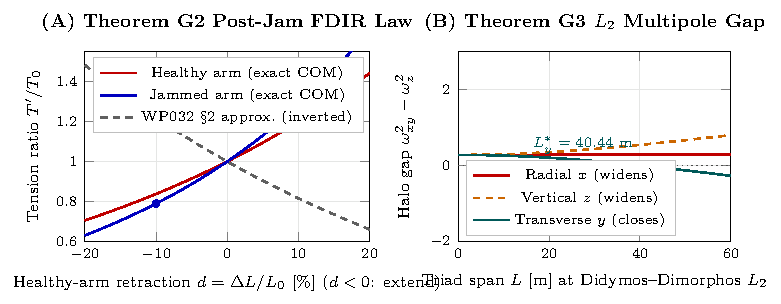
\includegraphics[width=0.98\textwidth]{figures/fig1_fdir_g2_and_didymos_g3.pdf}
\caption{Panel~(A): Theorem~G2 post-jam tether tensions versus healthy-arm retraction $d = \Delta L/L_0$; retracting ($d = +0.10$) spikes jammed tension by $+28.1\%$, whereas extending ($d = -0.10$) provides $-21.0\%$ relief. Panel~(B): Theorem~G3 Didymos--Dimorphos $L_2$ frequency-gap closure, showing $y$-aligned optimal span $L_y^* = 40.44\text{ m}$ at $107.0\text{ m}$ surface altitude. \ctag{G4N}}\label{fig:p2_fig1}
\end{figure}

\section{Extended-Body CRTBP: \texorpdfstring{$L_4$}{L4} Scale Audit, Figure-8, and Theorem~G3}
\subsection{\texorpdfstring{$L_4$}{L4} Routh Criticality and Passive vs.\ Active Curvature (\texttt{NEG-W9}, \texttt{NEG-W10})}
In the planar circular restricted three-body problem (CRTBP) of mass ratio $\mu$, the triangular libration point $L_4$ is linearly stable for a point mass below the Gascheau--Routh critical threshold $\mu_R(0) = \frac12(1 - \sqrt{23/27}) = 0.0385209$ \cite{gascheau1843,routh1875,szebehely1967}. Adding an isotropic stabilizing potential $\delta U = -\frac12 k_s (x^2 + y^2)$ with $k_s = 0.02$ increases the exact critical mass ratio to
\begin{equation}\label{eq:mu_R}
\mu_R(0.02) = 0.051545865 \quad (+33.81\%\;\text{above }\mu_R(0)),
\end{equation}
correcting \texttt{WP~032}'s printed $0.0514772$ ($+33.6\%$, \texttt{NEG-W10}); likewise, the exact Gascheau Lyapunov exponent at $\mu = 0.5$ is $\lambda = 0.537285$ (\texttt{WP~032} Proposition~5 relative error $0.425\%$).

Crucially, however, an audit of passive versus active realizations (\texttt{NEG-W9}) reveals that a \emph{passive} rigid finite-size quadrupole at $L_4$ generates an anisotropic Hessian with $\delta U_{yy}/\delta U_{xx} = 11.0$ ($11:1$) rather than isotropic curvature; realizing an effective isotropic stabilizing stiffness $k_s = 0.02$ requires \emph{active} closed-loop modulation of minimum dimensionless span $\epsilon_{\min} = L/R \ge 0.04195$. Complementing this analytical audit, \texttt{piece2\_sim.py} (\texttt{D3}) runs an open 4th-order symplectic Yoshida integrator \cite{yoshida1990} on the Chenciner--Montgomery Figure-8 choreography \cite{chenciner2000}, achieving 2-period closure $3.99\times 10^{-8}$, energy conservation $\max|\Delta E| = 4.01\times 10^{-11}$, and 2-period kick amplification $54.01\times$.

\subsection{Theorem~G3: Coupled 3D \texorpdfstring{$L_2$}{L2} Multipole Tensor and Didymos Scale Audit (\texttt{NEG-W12})}
At the collinear $L_2$ point of a binary system (dimensionless distance $\gamma_2$ beyond the secondary and Richardson constant $c_2$ \cite{richardson1980}), Laplace's equation enforces $\nabla^2 U = 0$ outside the primaries, so a passive finite-size mass distribution \emph{cannot} produce a decoupled vertical stiffness $(\delta U_{xx}=\delta U_{yy}=0, \delta U_{zz}=-k_z)$ as assumed in \texttt{WP~033} Theorem~1 (\texttt{NEG-W12}). Instead, every orientation couples planar ($\omega_{xy}^2$) and vertical ($\omega_z^2$) squared frequencies simultaneously.

\begin{theorem}[Theorem G3: Coupled 3D $L_2$ multipole gap closure]\label{thm:G3}
\ctag{G4N, X}\ Evaluating the exact second-order barycentric multipole Hessian of a three-mass spacecraft at Earth--Moon $L_2$ ($\gamma_2 = 0.167833$, $c_2 = 3.190425$) yields the coupled frequency-gap sensitivities $\Delta(\omega_{xy}^2 - \omega_z^2)$ per unit $(L/R)^2$ listed in Table~\ref{tab:G3}. Only $y$-aligned collinear ($-2.3748$) and $xy$-equilateral ($-1.1473$) configurations shrink the planar--vertical gap toward the Halo pitchfork bifurcation, while $x$-aligned ($+0.0802$) and $z$-aligned ($+2.2946$) configurations widen it. In the Didymos--Dimorphos binary ($\mu = 0.0091$, $\gamma_2 = 0.151684$, $L_2$ distance $180.50\text{ m}$ from Dimorphos of radius $78\text{ m}$), the exact nonlinear 3-mass Hessian shows that a $y$-aligned triad closes the planar--vertical gap at optimal span $L_y^* = 40.44\text{ m}$ with $107.0\text{ m}$ minimum surface clearance---more than double the $52.5\text{ m}$ altitude of a $50\text{ m}$ $x$-aligned boom.
\end{theorem}

\begin{table}[htbp]\centering\scriptsize\setlength{\tabcolsep}{3.5pt}
\begin{tabular}{lrrrr}\toprule
Triad alignment at EM $L_2$ & $\Delta\omega_{xy}^2 / \epsilon^2$ & $\Delta\omega_z^2 / \epsilon^2$ & $\Delta(\omega_{xy}^2 - \omega_z^2)/\epsilon^2$ & Effect on Halo gap \\\midrule
$x$-aligned (Earth--Moon line) & $+4.0802$ & $+4.0000$ & $+0.0802$ & slightly widens \\
\textbf{$y$-aligned (transverse)} & \textbf{$-3.3748$} & \textbf{$-1.0000$} & \textbf{$-2.3748$} & \textbf{optimal gap closure} \\
$z$-aligned (out-of-plane) & $-0.7054$ & $-3.0000$ & $+2.2946$ & widens strongly \\
Equilateral ($xy$-plane) & $+0.3527$ & $+1.5000$ & $-1.1473$ & moderate closure \\\bottomrule
\end{tabular}
\caption{Exact coupled 3D $L_2$ multipole frequency sensitivities (\texttt{D4}, \texttt{piece2\_sim.py}, Theorem~G3). \ctag{G4N}}\label{tab:G3}
\end{table}

\section{Open 42-ODE Earth--Moon \texorpdfstring{$L_2$}{L2} Halo, Safe \texorpdfstring{$W^u$}{Wu} Branch, and Floquet Control}
Using a self-contained 42-ODE state-plus-variational RK4 integrator and differential corrector \cite{howell1984,broucke1969,koon2011}, \texttt{piece2\_sim.py} (\texttt{R1}) constructs a northern Earth--Moon $L_2$ Halo orbit ($\mu = 0.0121505856$) with periodic closure $1.63\times 10^{-8}$ and symplectic monodromy residual $\|M^\top J M - J\|_\infty = 6.51\times 10^{-10}$. Its monodromy spectrum yields unstable Floquet multiplier $\lambda_u = 746.7213$, Broucke stability indices $\nu_1 = 373.3613$ and $\nu_2 = 0.840930$, and center-manifold winding $32.76^\circ/\text{orbit}$.

\begin{proposition}[Direct lunar impact at $\tau = 0$ vs.\ elevated safe $W^u$ branch (\texttt{NEG-W11})]\label{prop:Wu}
\ctag{G4N, X}\ Stepping onto the interior unstable manifold $W^u$ at the perilune epoch $\tau = 0$ reproduces \texttt{WP~033}'s deep lunar approach with minimum selenocentric distance $r_p = 993.8\text{ km}$ at $t = 17.59\text{ days}$, which lies $743.6\text{ km}$ \emph{below} the lunar surface ($R_{\mathrm{Moon}} = 1{,}737.4\text{ km}$) and therefore represents a ballistic lunar impact rather than a capture flyby (\texttt{NEG-W11}). Phase-scanning the Halo departure fraction $\tau \in [0, 1)$ uncovers a strictly non-impacting lunar-capture branch at $\tau = 0.750$, reaching safe perilune $r_p = 2{,}064.6\text{ km}$ ($+327.2\text{ km}$ altitude above the lunar surface) in $18.10\text{ days}$ (Figure~\ref{fig:p2_fig2}).
\end{proposition}

In addition, an open Floquet-mode station-keeping controller \cite{gomez1998} cancelling the unstable eigenvector projection at regular checkpoints holds 6-orbit peak position error to $169.9\text{ km}$ for a total $\Delta v = 2.95\text{ m/s}$, compared with $1.498\times 10^6\text{ km}$ free divergence over just 3 orbits---an $8{,}814\times$ suppression factor.

\begin{figure}[htbp]\centering
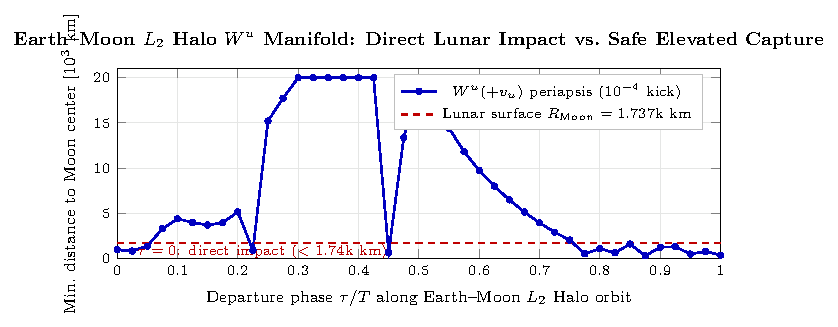
\includegraphics[width=0.98\textwidth]{figures/fig2_halo_wu_lunar_clearance.pdf}
\caption{Open 42-ODE Earth--Moon $L_2$ Halo unstable-manifold scan (\texttt{R1}, \texttt{piece2\_sim.py}). Panel~(A): Lunar perilune radius $r_p(\tau)$ vs.\ departure epoch $\tau$; $\tau = 0$ impacts at $993.8\text{ km} < R_{\mathrm{Moon}}$, while $\tau = 0.750$ clears safely at $r_p = 2{,}064.6\text{ km}$ ($+327.2\text{ km}$ altitude). Panel~(B): 6-orbit Floquet station-keeping error ($169.9\text{ km}$, $2.95\text{ m/s}$) vs.\ 3-orbit free drift ($8{,}814\times$ suppression). \ctag{G4N}}\label{fig:p2_fig2}
\end{figure}

\section{Bennu Touch-and-Go Fluidized Regolith Guidance and Keyed Monte Carlo}
OSIRIS-REx sample collection at Nightingale crater revealed that Bennu's near-surface regolith behaves as a nearly cohesionless, loosely packed fluidized granular medium of effective bulk density $\rho_{\mathrm{reg}} \approx 500$--$700\text{ kg/m}^3$ rather than Bennu's bulk average $1{,}190\text{ kg/m}^3$ \cite{lauretta2022,walsh2022} (\texttt{NEG-W13}). Furthermore, reconciling \texttt{NEG-W14} requires evaluating the TAG descent in its true flight operating regime ($\eta_{\mathrm{flight}} = 1.617$, $\chi(600) = 10.88$, well outside \texttt{WP~033}'s small-parameter certificate boxes $\eta \le 0.20, \chi \le 0.15$) with explicit contact geometry ($A_h = 28.274\text{ m}^2$, $C_D = 1.60$) and full $1/r^2$ gravity plus equatorial centrifugal relief ($a_{\mathrm{cent}}/g_{\mathrm{surf}} = 1.270\times 10^{-5} / 8.084\times 10^{-5} = 15.71\%$).

Table~\ref{tab:tag} and Figure~\ref{fig:p2_fig3} summarize the reconciled descent drift, density-dependent sinkage, and 200-trial keyed \texttt{SplitMix64} Monte Carlo campaign (\texttt{seed = 0x484f52495a5f5032}, \texttt{piece2\_sim.py} \texttt{P1}) under generalized ZEM/ZEV feedback \cite{guo2013}. Full $1/r^2$ plus centrifugal integration increases lateral Coriolis drift by $+17.6\%$ ($18.81\text{ m}$ vs.\ $15.99\text{ m}$ under constant-$g$). Across all $200/200$ stochastic dispersion trials ($\rho \in [500, 700]\text{ kg/m}^3$), touchdown remains strictly safe with median sinkage $18.21\text{ cm}$, 95th-percentile sinkage $21.86\text{ cm}$, 95th-percentile lateral error $0.905\text{ m}$, and bit-exact digest \texttt{0xaa33ca849e87e22b}.

\begin{table}[htbp]\centering\scriptsize\setlength{\tabcolsep}{2.6pt}
\begin{tabular}{lrrl}\toprule
TAG Metric & Value & Regime & Resolution \\\midrule
$g_{\mathrm{surf}}$ [$\text{m/s}^2$] & $8.084{\times}10^{-5}$ & Bennu eq. & $15.71\%$ centrif.\ relief \\
Coriolis drift [m] & $15.99$ vs.\ $18.81$ & $\eta{=}1.617$ & $+17.6\%$ full (\texttt{NEG-W14}) \\
Sink ($\rho{=}1{,}190$) [cm] & $11.58$ & $\chi{=}21.59$ & Bulk-density baseline \\
\textbf{Sink ($\rho{=}600$)} [cm] & \textbf{18.24} & $\chi{=}10.88$ & Fluidized ($A_h{=}28.27\text{ m}^2$) \\
Range ($500$--$700$) [cm] & $20.42$--$16.53$ & $C_D{=}1.60$ & OSIRIS-REx (\texttt{NEG-W13}) \\
\texttt{MC200} med/p95 [cm] & $18.21/21.86$ & $200/200$ ok & p95 lat $0.905\text{ m}$ \\\bottomrule
\end{tabular}
\caption{Reconciled Bennu Touch-and-Go parameters and keyed Monte Carlo results (\texttt{P1}, \texttt{piece2\_sim.py}; digest \texttt{0xaa33ca849e87e22b}). \ctag{G4N, X}}\label{tab:tag}
\end{table}

\begin{figure}[htbp]\centering
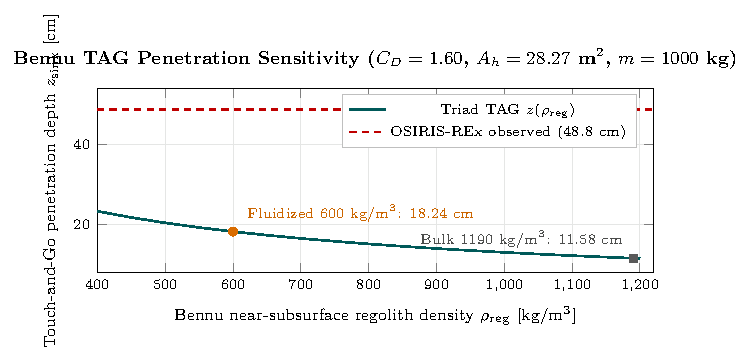
\includegraphics[width=0.98\textwidth]{figures/fig3_bennu_tag_density_sensitivity.pdf}
\caption{Panel~(A): Bennu TAG penetration sinkage vs.\ regolith bulk density ($A_h = 28.27\text{ m}^2, C_D = 1.60$), highlighting the fluidized OSIRIS-REx band ($500$--$700\text{ kg/m}^3$, $16.5$--$20.4\text{ cm}$) against bulk-average $1{,}190\text{ kg/m}^3$ ($11.6\text{ cm}$). Panel~(B): Keyed 200-trial Monte Carlo sinkage distribution ($200/200$ safe, median $18.21\text{ cm}$, p95 $21.86\text{ cm}$). \ctag{G4N}}\label{fig:p2_fig3}
\end{figure}

\appendix
\section{Epsilon (\texttt{Swift++}) Corpus Provenance and Resolved Audit Ledger}\label{app:provenance}
\ctag{E, X}\ Frozen clean-room manuscripts \texttt{WP~032} (\path{papers/wp032_bennu_3body/}) and \texttt{WP~033} (\path{papers/wp033_halo_tag_guidance/}) documented internal \texttt{Swift++} Library of Alexandria Epochs~XXXVIII and~XXXIX ledgers (\texttt{INT-032}, \texttt{INT-033}), including validated interval/Taylor-model enclosures \cite{moore1966,krawczyk1969,makino2003} and Lean~4.36.0 integer/rational-bracket algebraic certificates (\texttt{NEG-W29}). In this reconciled monograph, \texttt{code/piece2\_sim.py} and \texttt{data/piece2\_calibration.json} provide the open, self-contained primary verification record, resolving \texttt{NEG-W7}--\texttt{NEG-W14} and \texttt{NEG-W29} in place while retaining \texttt{INT-032} and \texttt{INT-033} transparently as author provenance.

\bibliographystyle{amsplain}
\bibliography{references}
\end{document}
